% !TEX root = main.tex

\chapter{Existing experimental system}
The work developed in this thesis lies on top of an existing experiment. In this chapter we are going to describe the essential parts of the already existing setup on top of which the addressing system has been build. Calcium-40 ions are used in the experiment, the implementation of several techniques for
trapping and manipulating these ions are discussed. Furthermore, the addressing setup utilizes 393 nm light, the laser emitting this light was already installed and used, thus that setup is presented. The experiment can be controlled remotely via computers, an overview of how it is implemented and how it works is also given.

\section{Ion trap and key techniques}
\subsection{Calcium Ions}
\label{sec:calciumion}
\begin{figure}
\centering
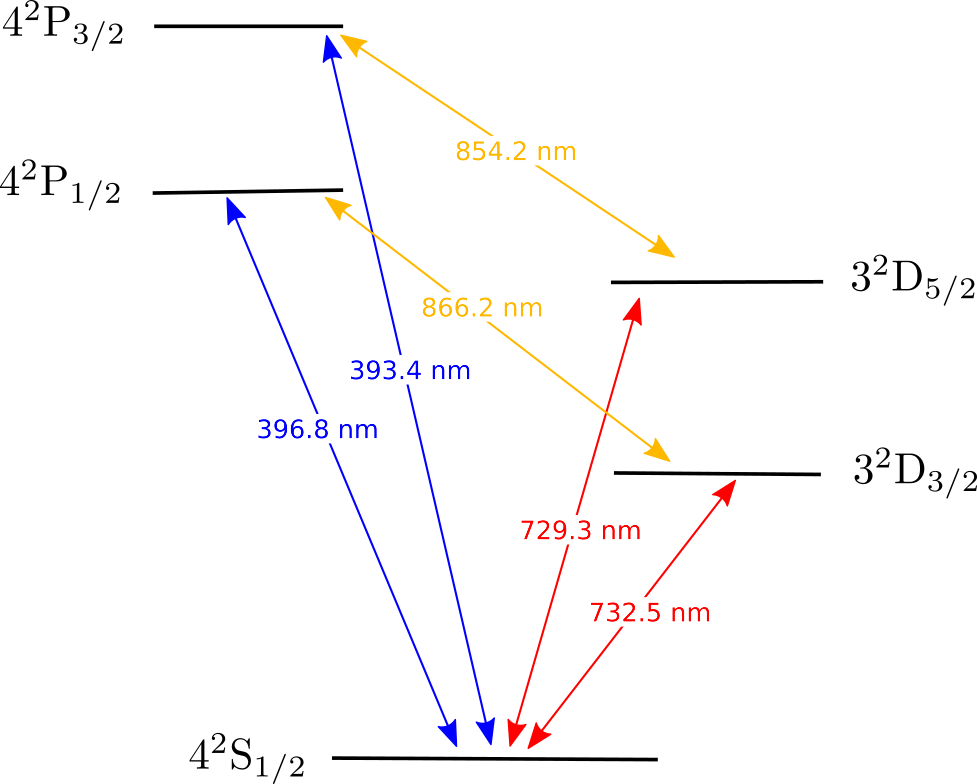
\includegraphics[width = .6 \textwidth]{calciumscheme}
\caption{Level scheme of $^{40}\text{Ca}^+$ with main transitions highlighted. Blue transitions are dipole transitions suitable for cooling, imaging and photon detection. Red transitions are dipole forbidden, but accessible with electric quadrupole, they are used to encode qubits. Orange transition are usually repumped. In addition, the 854 nm transition is tuned in resonance with the cavity for photon generation purposes. From more and precise value see table \ref{transitiontable}}
\label{calciumscheme}
\end{figure}
In choosing the appropriate ion to trap, one looks first of all for simplicity, which means choosing an element with one single electron in the most outer orbital.
This fact limits the choice to the second group of the periodic table, many of these elements has been successfully trapped: beryllium \cite{beryllium}, barium \cite{barium}, strontium \cite{strontium}, and calcium \cite{calcium}.
The latter has been chosen for this experiment, as calcium has transitions easily accessible with commercial diode and titanium-sapphire lasers. The most abundand isotope of calcium is calcium-40, which is a common choice, but not the only one \cite{Tanaka2007}. Nevertheless, $^{40}\text{Ca}^+$ ions were our choice. In figure \ref{calciumscheme} the level scheme of the only electron in the outer shell is presented. A single ground state is present $\text{S}_{1/2}$ with no hyperfine structure as $^{40}\text{Ca}^+$ does not posses a nuclear spin. There are two short lived excited states ($\sim 7$ ns): $\text{P}_{1/2}$, and $\text{P}_{3/2}$ which are accessible with dipole transitions. These states have different decay channel, for $\text{P}_{1/2}$
the branching ratios are $6\%$ to $\text{D}_{3/2}$, and $94\%$ back to the ground state. For  $\text{P}_{3/2}$ there is a probability of $5.3\%$ to decay to   $\text{D}_{5/2}$, $0.6\%$ to go to  $\text{D}_{3/2}$ and $94\%$ to return to  $\text{S}_{1/2}$. Due to the short lifetimes of these two states, they are suitable for laser cooling and state detection, while the states $\text{D}_{3/2}$ and $\text{D}_{5/2}$
are metastable ($\sim 1$ s) since accessible with electric quadrupole transition. Since the lifetime of the D states are much greater than typical coherence time, they can encode a stable qubit and manipulated without worrying about dissipative process. Table \ref{transitiontable} summarizes details about the different transitions, and what they are used for. A more detailed description and implementation is discussed in the next section.

\begin{table}[H]
\centering
\begin{tabular}{c c c c c}
 \toprule
    {Transition} & {wavelength (nm)} & {Decay rate $\Gamma$} & Lifetime $\tau$ & {Main use} \\ \midrule
   $\text{S}_{1/2} \to \text{P}_{1/2}$ & 396.847 & $2\pi \times 20.8$ MHz & 7.7 ns &  Cooling and imaging \\
    $\text{S}_{1/2} \to \text{P}_{3/2}$  & 393.366 & $2\pi \times 21.4$ MHz & 7.4 ns & Photon generation\\ \midrule
   $\text{S}_{1/2} \to \text{D}_{3/2}$ & 732.389 & $2\pi \times 0.132$ Hz & 1.080 s & - \\
    $\text{S}_{1/2} \to \text{D}_{5/2}$  & 729.147 & $2\pi \times 0.136$ Hz & 1.045 s   & Qubit  \\\midrule
    $\text{P}_{1/2} \to \text{D}_{3/2}$  & 866.214 &  $2\pi \times 1.70$ MHz  &  94.3 ns  & Repumping \\
    $\text{P}_{3/2} \to \text{D}_{5/2}$  & 854.209 & $2\pi \times 1.34$ MHz & 101 ns  & Cavity photon  \\
    $\text{P}_{3/2} \to \text{D}_{3/2}$  & 849.802 & $2\pi \times 1.52$ MHz  & 902 ns   & Repumping \\ \bottomrule
\end{tabular}
\caption{Transitions in $^{40}\text{Ca}^+$ and current use in the experiment. Values are taken from \cite{ion_spacing,stute}}
\label{transitiontable}
\end{table}

-- Add lasers direction!

\subsection{Trapping, cooling, and state readout}
\begin{figure}
\centering
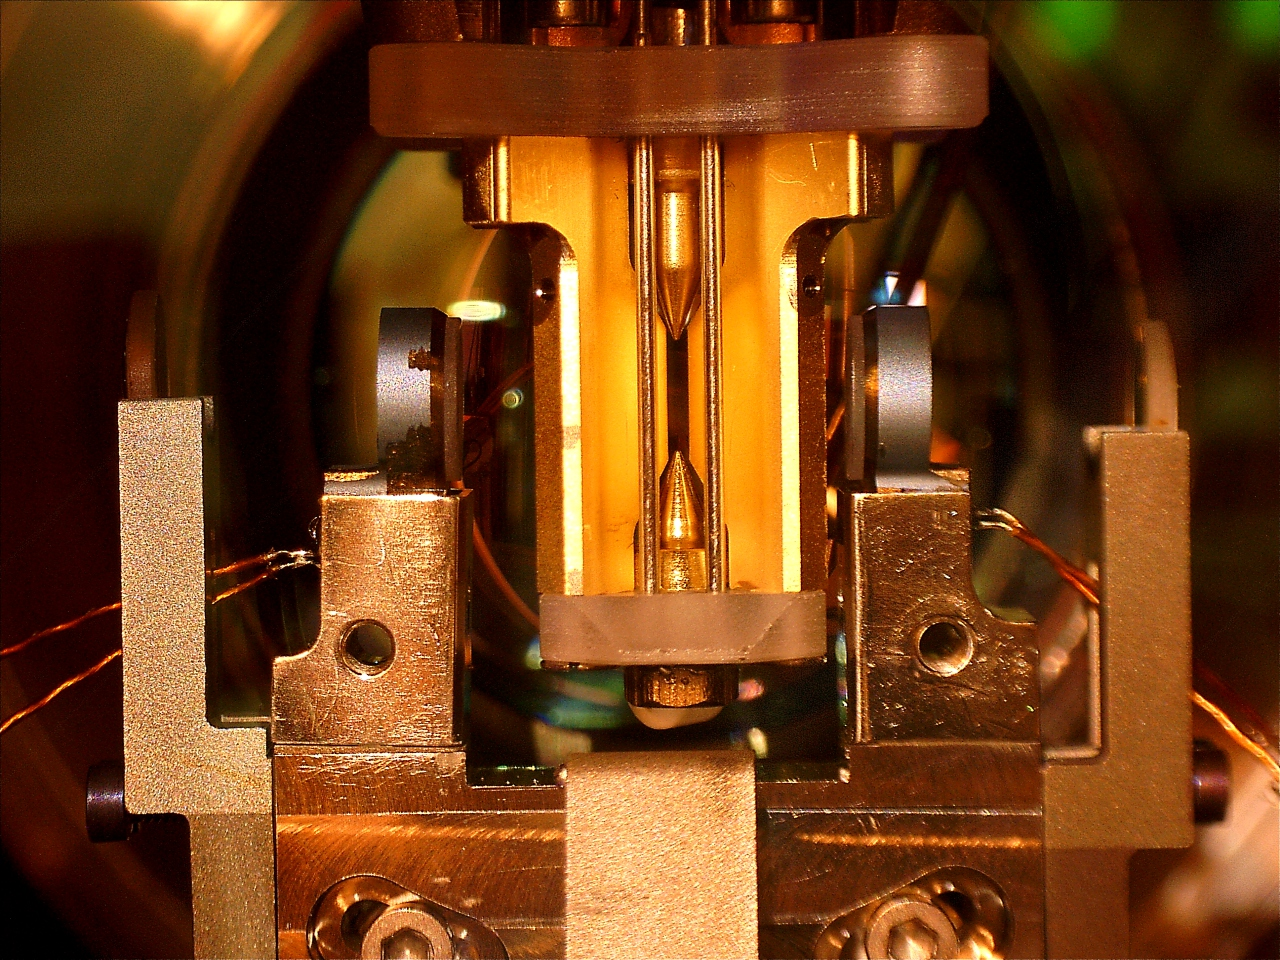
\includegraphics[width = .7\textwidth]{phototrap}
\caption{Photo of the mounted trap, a pair of compensation electrodes and the mirrors of the cavity are also visible.}
\label{trapphoto}
\end{figure}
Our trap is a linear 3D RF Paul trap as depicted in figure (), the picture of the real trap is displayed in figure \ref{trapphoto}. The trap consists of 4 ortoghonal electrodes with blade shape for RF confinement in the radial direction. In the axial direction confinement is achieved with two tip electrodes that forms the endcaps. Everything is made in titanium, it is covered in gold and the trap itself is mounted vertically on a Shappire holder. The endcaps are 5 mm apart, and they are usually kept at a voltage in the order of 500-1000V, which means an axial frequency of $\omega_z \sim 2\pi \times 0.7-1$ MHz. The four blades are 0.8 mm from the center of the trap and driven with an RF of $\sim 24$ MHz. Due to the high power delivered to this blades ($\sim-4$ dBm), the RF signal has to be impedance matched with the trap, this is done with an helical resonator.
The trap also includes three pairs of compensations electrodes that can be used to compensate micromotion.
Loading of ions is done with an atomic oven, calcium is heated a directed towards the trap, in the trap the atoms undergo 2-stage photon ionization. The first laser 375 nm, excite one electron to a very high excited state, the second laser 422 nm, brings the electron to free space ionizing the atom. Such two stage process allows to filter for isotopes and ionize only $^{40}\text{Ca}$. Loading usually takes minutes or tens of minutes depending on the number of ions one wants to load. Storing time can be in the order of days, especially when a single ion is loaded.\\
Once loaded, ions are laser cooled with 397 nm light on the transition $\text{S}_{1/2} \to \text{P}_{1/2}$ detuned at $-\Gamma/2$. An additional repumper on the transition $\text{P}_{1/2} \to \text{D}_{3/2}$ is also used to avoid for the electron being stuck in the $\text{D}_{3/2}$ state. For typical experiment a stage of doppler cooling is always included, this lasts from 1 millisecond up to tens of milliseconds.\\
With the same Doppler cooling light, imaging can also be done. The light shines on the ions exciting the transition $\text{S}_{1/2} \to \text{P}_{1/2}$ driving the electron to the excited states which then decay spontaneously emitting a photons. Photon are collected with a custom objective with NA of $\sim 0.3$, which means an efficiency of 2.5 \% over the solid angle $4\pi$. The objective focuses the collected photons 1.5 meters away where a CCD camera (Andor iXon Ultra 897) is placed. The geometrical path of the imaging is displayed in figure \ref{imgsetup}, this setup has a magnification factor of $\sim$18.6. The same objective is also used for the addressing setup built within this thesis. Therefore, the imaging optical path must be partially shared with the newly built addressing. In depth overview of objective is therefore given in section \ref{sec:obj}.\\
State read out is possible with this kind of imaging, with the difference of using a photonmultiplier tube (PMT) for counting photons instead of a camera. Consider a qubit encoded in the states $\text{S}_{1/2} \to \text{D}_{5/2}$, if the imaging laser is switched on, the electron will be projected either to the $\text{S}_{1/2}$ level or in the $\text{D}_{5/2} $. In the first case, photons are scattered from the ion and collected on the PMT, in the second case the electron is shelved and will not scatter any photon. Hence, the two cases are distinguishable by counting statistics. An histogram can be constructed  with the number of photon measured, and a properly set threshold differentiates between bright and dark states. Typical detection times are in the order of milliseconds.

\begin{figure}
\centering
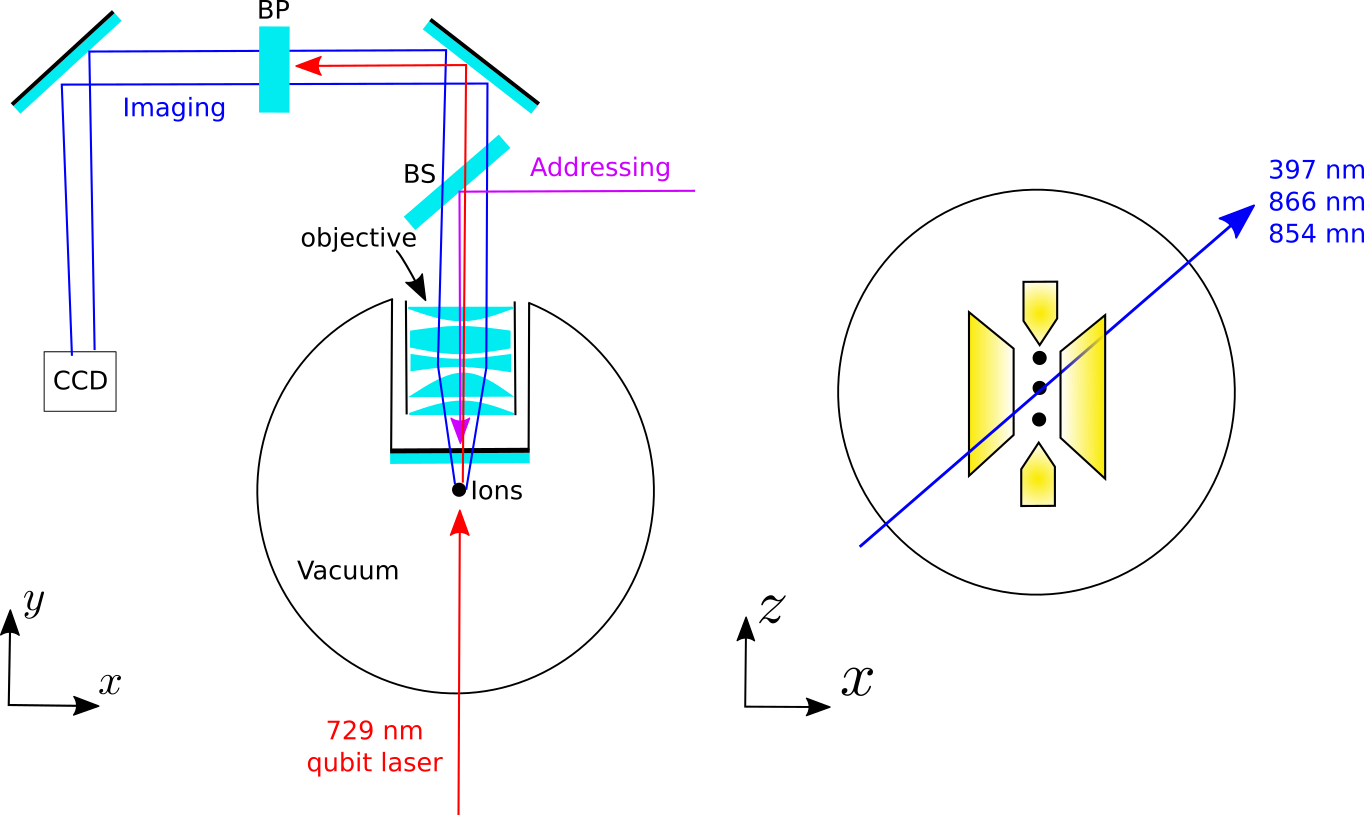
\includegraphics[width = .6\textwidth]{imgsetup}
\caption{Top view of the imaging optical path, the objective collimates and focuses the scatter photons onto the CCD camera. The addressing setup must share part of this path, as the same objective is used for focusing.}
\label{imgsetup}
\end{figure}

\section{393 nm laser}
\begin{figure}
\centering
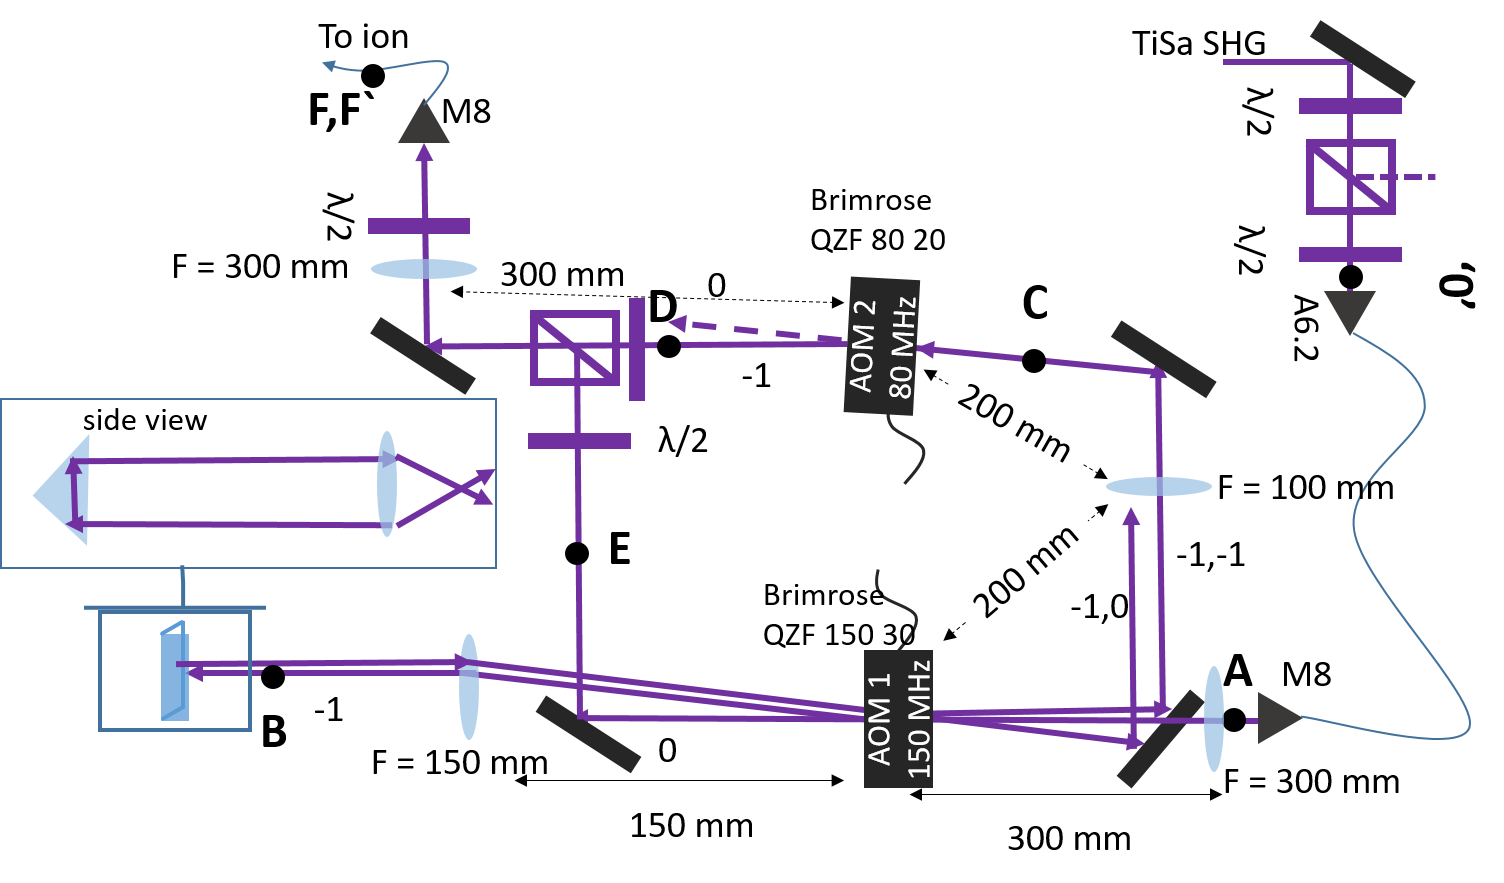
\includegraphics[width = .9\textwidth]{scheme393}
\caption{393nm laser optical setup. Two paths are present, a resonant one, and a detuned that goes through two AOM's.}
\label{scheme393}
\end{figure}
The laser used to drive the Raman transition is 393 nm. This light is obtained from a titanium-sapphire laser from MSquared. The laser is optically pumped with 8 W of light at 532 nm coming from a Lighthouse Photonics Sprout laser. The active Ti:Sa crystal is contained in a cavity in a bow tie configuration, together with an optical diode, etalon, birefringent mirror, and tunable cavity mirror for frequency tuning and stabilization. The fundamental mode is at 786 nm with tunability ranging from 725 nm to 875 nm that can be controlled remotely on the computer. The laser can also be locked to a wavemeter and tuned with it.
The fundamental light is frequency doubled to 393 nm via a MSquared ECD-X external cavity resonant doubler accessory module. Blue light can be obtained with up to 1 W of power. Before reaching the ion trap, 393 nm light is sent through the setup in figure \ref{scheme393}. There are two AOM's in the setup, AOM1 from Brimrose with a working frequency of 150 MHz, AOM2 is still from Brimrose and works at 80 MHz. There are two paths for the light: a resonant one which gets resonant light from the laser, and send it directly to the ion. This path is the zeroth order of AOM1, light is not diffracted, but it is coupled to a fiber using a PBS, and then goes to the ion trap. The second path is the detuned one, the main purpose is to red detune the laser light in order to excite the Raman transition. This path goes through both AOM's, the first AOM1 is in double pass configuration and shift the light by 300 MHz. Diffracted light in the -1 order is sent through and reflected back again in the same AOM by a prism. Diffracted light from AOM1 is sent to the second AOM used in single pass configuration which further shift the light by 80 MHz. The diffracted light (-1 order), from AOM2, is coupled to a fiber that brings it to the ion trap. The detuned beam therefore reaches the ion with a -380 MHz detuning which can be modulated within the bandwidths of both AOM's. The zeroth order of AOM2 is blocked to avoid that this light is coupled to the fiber and end in the trap. Lenses in the setup have the purpose to focus the waist of the beam in the AOM's aperture avoiding unwanted beam steering and therefore losing coupling to the fiber.
AOM2 is also used to generate a bichromatic field, simply by driving this AOM with a multifrequency signal.\\
This particular setup had to be altered after the installation of the addressing setup, minor adjustment had to be made in order to compensate for an additional frequency shift due to the AOD in the addressing setup. AOM2 was switched from -1 order to +1 order, and driving frequency were changed to 180 MHz for AOM1 and 70 MHz for AOM2.

\section{Experiment control}
Complex experiments require control over a large network of AOM's and other devices. Furthermore, laser pulse coherence is also fundamental in some sequential experiment. The need of fast and coherent pulse control is fulfilled by an electronic system that can be controlled with a software on a computer where every device connected to the network can be controlled. The experiment control network is sketched in figure \ref{expcontrol}. On the computer TrICS software is installed, this computer is connected to a BUS system with a NIDAQ card. Direct Digital Synthesizers (DDS) used to generate radio frequency signal for AOM's are connected to the BUS system through an optocoupler to avoid ground loops. Therefore, the computer can send electric signal over the BUS to specific DDS allowing for direct control. The computer is also connected via ethernet to a Pulse Box, and through another NIDAQ card to the same box. The card sends and receive trigger signals, while over the ethernet, sequences are uploaded. The pulse box contains DDS and and FPGA, thus it has the capabilities of generating short and coherent TTL pulses ($\mu$s) that can send to TTL switches placed between a DDS, the source of the signal, and an AOM. The Pulse Box contains fast switching DDS, this means that the frequency of such DDS can be changed quickly, unlike the DDS on the BUS. The whole system runs with two separated clocks, one at 10 MHz, and another one at 1.2 GHz.\\
With this system, a laser pulse can be controlled in frequency, amplitude, and length. Frequency and amplitude are set in the DDS by sending a signal over the BUS system to th appropriate DDS channel. The length of the pulse can be controlled precisely by the Pulse Box. Moreover, the Pulse Box also has pulse shaping possibilities.\\
In a typical experiment, a sequence of pulses is programmed in python on the computer. When the experiment is run, the computer uploads the sequence to the FPGA inside the Pulse Box. Next, the computer updates the DDS on the BUS with the appropriate values for the experiment, sends a trigger signal to the Pulse Box and the Pulse Box generates and sends all the signals for the sequence. When the experiment is done, the Pulse box sends another trigger back to the computer, which proceeds to prepare for the next measurement point, it updates the values of the BUS DDS, reupload the code to the Pulse Box, sends a trigger to start the sequence and the loop is repeated.

\begin{figure}
\centering
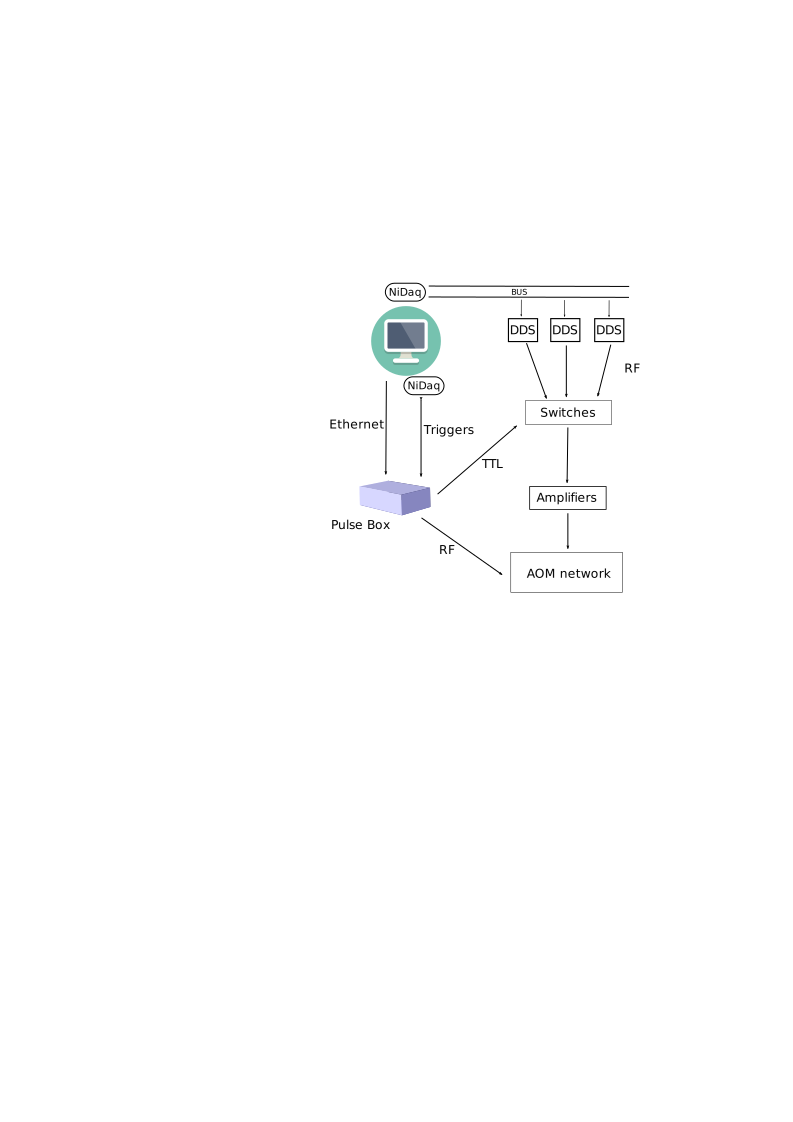
\includegraphics[width =.5\textwidth]{expcontrol}
\caption{Schematic of the experimental control. Everything is controlled remotely by a pc. During a sequence a pulse box generated coherent pulses to the appropriate devices.}
\label{expcontrol}
\end{figure}

\begin{figure}
\centering
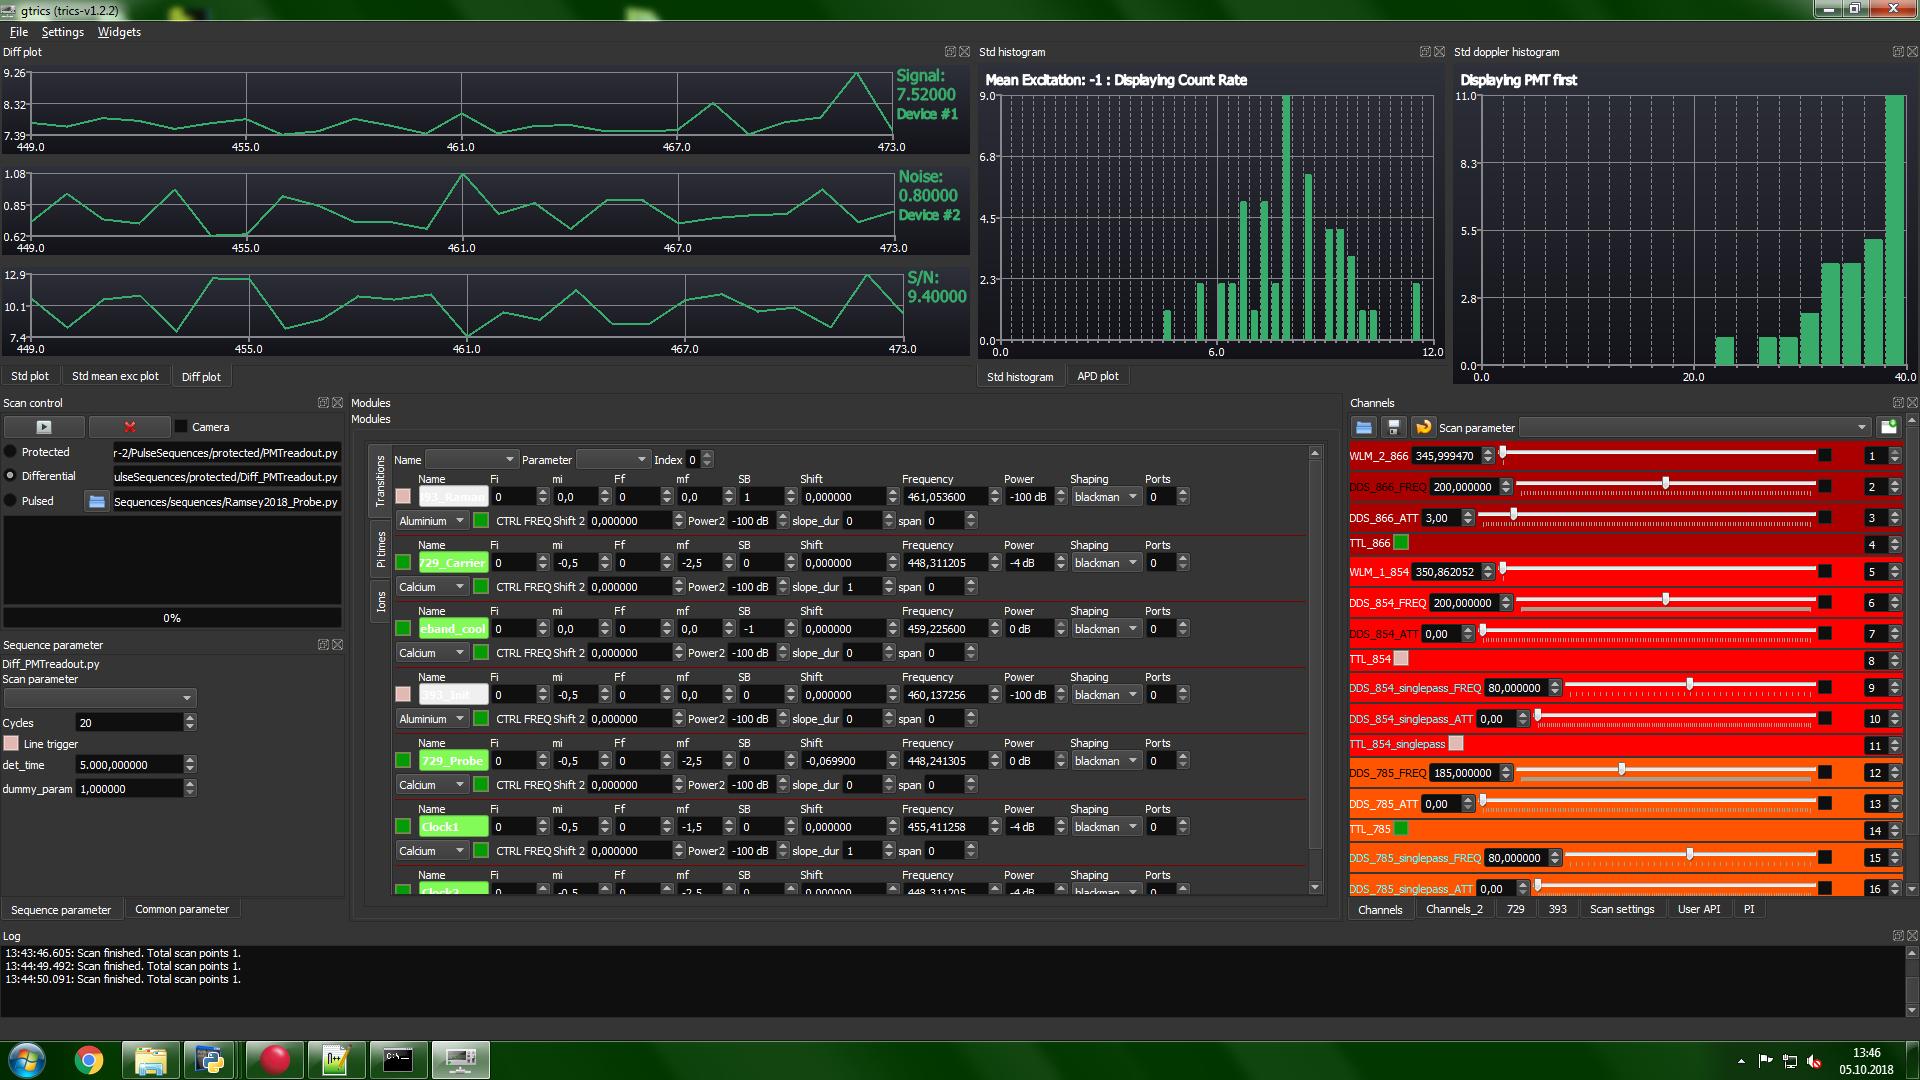
\includegraphics[width =\textwidth]{trics}
\caption{Trics software used to change all the experiment parameters and launch measurements.}
\label{trics}
\end{figure}
